\documentclass[Screen16to9,17pt]{foils}
\usepackage{zencurity-slides}
\externaldocument{SDL-practices-exercises}
\selectlanguage{english}




% Secure Development Practices
% Contents

%


\begin{document}

\mytitlepage
{0. Introduction}
{Secure Development Practices}

\hlkprofiluk

\slide{Goals for today}

 \hlkimage{4cm}{thomas-galler-hZ3uF1-z2Qc-unsplash.jpg}

Todays goals:
\begin{list2}
\item Overview, what is software security and vulnerabilities
\item Security patterns, insecure and secure design
\item What is SDL, SDLC, SSDL -- multiple names, but essentially the same
\item Security Testing Versus Traditional Software Testing
\item Standards ISO27001/CIS Controls, Application Software Security
\end{list2}

  Photo by Thomas Galler on Unsplash

\slide{Software Security}

\hlkimage{10cm}{software.pdf}

\begin{list1}
\item Software security - because software is everywhere
\item Give a high level view -- don't try to remember everything just yet
\end{list1}


\slide{Contents Day 0}

\begin{list2}
\item Software security in general -- how do things fail
\item History, cases, vulnerabilities, falsehoods and assumptions
\item Security principles: least privilege, fail-safe defaults, etc.
\item OWASP Top 10, CVE/WCE and "Monster mitigations"
\item Security patterns, insecure and secure design
\item Policies, coding standards, compiler warnings, git hooks, defensive programming
\item Code-Auditing Strategies: static analysis and dynamic analysis
\item Security Testing Versus Traditional Software Testing
\item Secure Development Lifecycle (SDL, SDLC, SSDL) -- multiple names, but essentially the same
\item Standards ISO27001/CIS Controls, Application Software Security
\item Optional: Exercises, questions
\end{list2}


Day 1 will be Advanced subjects and details



\slide{Time schedule Day 0}

Plan for the day
\begin{list1}
\item 09:00 - 09:45 -- Session 0: How software fails
\item 10:00 - 10:45 -- Session 1: How does \emph{bad software} happen?!
\item 11:00 - 11:45 -- Session 2: Security principles and design
\item 11:45 - 12:30 -- Lunch
\item 12:30 - 13:15 -- Session 3: Code auditing, analysis and security testing
\item 13:30 - 14:15 -- Session 4: Coding standards, Git hooks and scanner tools
\item 14:30 - 15:15 -- Session 5: Secure Development Lifecycle and standards
\item 15:30 - 16:00 -- Optional: Exercises, questions
\end{list1}


\slide{Session 0: How software fails}
\begin{list2}
\item Software security in general -- how do things fail
\item History, cases, vulnerabilities, falsehoods and assumptions
\item What is a CVE
\vskip 1em
\item Exercise: browse CVE sites, find vulnerabilities in software you use
\end{list2}


\slide{Computer worms}

\begin{quote}
A \emph{computer worm} is a program that copies itself from one computer to another.
\end{quote}
Source: \emph{Computer Security: Art and Science}, Matt Bishop, ISBN 9780321712332

\begin{list2}
\item Computer worms have existed since research began in the mid-1970s
\item Morris Worm from November 2, 1988 was a famous example
\begin{list2}
\item Often quoted: 6,000 of 60,000 computers infected -- but this was a guess,\\
other estimates are 1,000--3,000
\item Led to the creation of CERT/CC, and Morris was the first person tried under the Computer Fraud and Abuse Act
\end{list2}
\vskip 1em
\item Virus, trojan or worm?\\
Unless you work specifically in the computer virus industry, call it all malware
\end{list2}

\slide{The Internet Worm 2 November 1988}

{\renewcommand{\arraystretch}{1.6}
\begin{tabularx}{\textwidth}{|l|X|}\hline
{\bf Vulnerability} & {\bf How the worm abused it} \\\hline
Buffer overflow in fingerd & VAX code sent to overflow the buffer \\\hline
Sendmail & DEBUG functionality \\\hline
Trust between systems: rsh, rexec, ... & Found systems to infect in /etc/hosts.equiv, .rhosts, .forward, netstat ... \\\hline
Bad passwords & Password cracking using internal list of 432 words and /usr/dict/words \\\hline
\end{tabularx}}

\vskip 1em
\begin{list1}
\item Contained camouflage! Program name set to 'sh', used fork() to switch PID regularly
\item Made by Robert T. Morris, Jr.
\end{list1}

Source: \emph{The Internet Worm Program: An Analysis}, Eugene H. Spafford,\\
Purdue Technical Report CSD-TR-823, 1988\\
{\footnotesize\link{https://spaf.cerias.purdue.edu/tech-reps/823.pdf}}


\slide{Stuxnet}

\begin{list1}
\item Worm in 2010 intended to infect Iran nuclear program
\item Target was the uranium enrichment process
\item Infected other industrial sites
\item SCADA, and Industrial Control Systems (ICS) are becoming very important for whole countries
\item A small \emph{community} of consultants work in these \emph{isolated} networks, but can be used as infection vector - they visit multiple sites
\item More information can be found in \url{https://en.wikipedia.org/wiki/Stuxnet}
\end{list1}

Mentioned here as example of airgapped/isolated control networks

\slide{Current events}

Current events are always relevant, as they happen -- right NOW!
\begin{list2}
\item Fortinet CVEs - summary, make this as an exercise, evaluate a new product suggested by your boss
\item VPN -- protocols belong in network courses, but implementation is at least as important?
\item NIS2 -- impact on "software security", can you run an open source project with high risk CVEs?
\item Citrix ADC load balancers are popular in Denmark
\item OpenSSH even has security vulnerabilities -- coming from the OpenBSD project which focus on security
\item CPE routes hacked and become botnet devices
\end{list2}

This slide was written a long time ago! This last month both NetScaler and OpenBSD had new vulns!

\slide{Vulnerabilities - CVE}

\begin{list1}
\item Common Vulnerabilities and Exposures (CVE):
  \begin{list2}
  \item classification
  \item identification
  \end{list2}
\item When discovered each vuln gets a CVE ID
\item CVE maintained by MITRE - not-for-profit
org for research and development in the USA.
\item National Vulnerability Database search for CVE.
\item Sources: \link{http://cve.mitre.org/} og \link{http://nvd.nist.gov}
\item also checkout OWASP Top-10 \link{http://www.owasp.org/}
\end{list1}


\slide{Current CVEs}

We will be talking about software "problems" often named vulnerabilities, with CVE IDs
Here are some example vulnerabilities Rezilion identified back in 2023:
\begin{quote}
\begin{list2}
\item CVE-2026-45586 – CTFMON EoP, public zero-day
\item CVE-2026-41089 – Netlogon RCE CVSS 9.8, disclosed May, confirmed exploited in June
\item CVE-2026-56155 – AD FS EoP, exploited zero-day
\item CVE-2026-56164 – SharePoint EoP, exploited zero-day
\item CVE-2026-81963 – Windows Update Stack EoP, CVSS 7.8, on CISA KEV
\item CVE-2026-85880 – Windows ALPC heap overflow EoP, CVSS 7.8, AppContainer sandbox escape, on CISA KEV
\item CVE-2026-69730 – Windows DNS Server RCE, use-after-free, CVSS 9.8
\end{list2}
\end{quote}

Note: we will NOT dive deep into these, just acknowledge that they exist
%Source:\\ {\scriptsize


\slide{Microsoft Patch Tuesday: June--September 2026}

\begin{tabularx}{22cm}{|X|r| r|r|r|}\hline
Month & CVEs (Microsoft) & Critical & Zero-days & Exploited \\\hline
June  & 198--208  & 32--37 & 3 & 0 at release$^{*}$ \\\hline
July  & 569--570  & 56--59 & 3 & 2 \\\hline
August & 398--421 & 42--62 & 1--3 & 1 \\\hline
September & 964--974 & 50--113 & 2 & 2 \\\hline
\end{tabularx}

\begin{list2}
\item Vendor counts disagree by month; the ranges above reflect Microsoft's own bulletin count versus third-party trackers (Tenable, BleepingComputer, N-able, Krebs on Security, Qualys, Lansweeper)
\item Broader trackers that fold in republished third-party and Chromium-based Edge CVEs report far higher totals for the same months, e.g.\ ZDI counted 571 CVEs for June and 621 for July when Chromium fixes are included; Rapid7 counted 999 for September including 25 non-Microsoft CVEs
\item September's release is the largest in Patch Tuesday history, surpassing July; AI-assisted vulnerability discovery is cited as a factor in the increased volume
\item ZDI: 2,760 Microsoft CVEs patched so far in 2026 -- more than double any previous full year
\end{list2}

\slide{Microsoft Patch Tuesday -- June 2026}
\begin{list2}
\item 198--208 CVEs, 32--37 critical, 3 zero-days, none exploited at release
\item \emph{CVE-2026-45586} -- CTFMON EoP, public zero-day
\item \emph{CVE-2026-41089} -- Netlogon RCE CVSS 9.8, disclosed May, confirmed exploited in June
\end{list2}

\slide{Microsoft Patch Tuesday -- July 2026}
\begin{list2}
\item 569--570 CVEs, 56--59 critical, 3 zero-days, 2 exploited
\item \emph{CVE-2026-56155} -- AD FS EoP, exploited zero-day
\item \emph{CVE-2026-56164} -- SharePoint EoP, exploited zero-day
\item Largest Patch Tuesday release at the time, AI-assisted vulnerability discovery cited as a factor
\end{list2}

\slide{Microsoft Patch Tuesday -- August 2026}
\begin{list2}
\item 398--421 CVEs, 42--62 critical, 1 exploited zero-day
\item \emph{CVE-2026-68820} -- afd.sys (WinSock) EoP, CVSS 7.0, on CISA KEV\\
\link{https://www.tenable.com/blog/microsofts-august-2026-patch-tuesday-addresses-398-cves-cve-2026-68820}\\
Exercise -- check if any of these still affect your organizations
\item Vendor counts disagree by month -- Microsoft's own bulletin count vs.\ third-party trackers
\end{list2}

\slide{Microsoft Patch Tuesday -- September 2026}
\begin{list2}
\item 964--974 CVEs, 50--113 critical, 2 exploited zero-days -- largest Patch Tuesday ever
\item \emph{CVE-2026-81963} -- Windows Update Stack EoP, CVSS 7.8, on CISA KEV
\item \emph{CVE-2026-85880} -- Windows ALPC heap overflow EoP, CVSS 7.8, AppContainer sandbox escape, on CISA KEV
\item \emph{CVE-2026-69730} -- Windows DNS Server RCE, use-after-free, CVSS 9.8, unauthenticated, not exploited at release\\
\link{https://www.tenable.com/blog/microsofts-september-2026-patch-tuesday-addresses-964-cves-cve-2026-81963-cve-2026-85880}
\item Out-of-band update needed days later: the patches broke Remote Desktop Services, Hyper-V Linux VMs and USB audio
\end{list2}

\slide{Not just Microsoft}
\begin{list2}
\item Microsoft is a well-known vendor here, but far from the only vendor with high numbers
\item \emph{Linux kernel} -- 5{,}681 CVEs in 2025 (highest single year ever recorded); already 2{,}308 CVEs in H1 2026, the single highest vendor count for the period\\
\link{https://linuxiac.com/linux-tops-2026-cve-charts/}
\item \emph{Fortinet} -- 27 new CVEs disclosed in a single two-day stretch in April 2026 across FortiOS, FortiSandbox, FortiWeb and more, several critical/unauthenticated\\
\link{https://www.greenbone.net/en/blog/fortinet-rce-vulnerabilities-2026-critical-vulnerabilities-in-fortisandbox/}
\item Other vendors worth showing: \emph{Oracle} (1{,}235 CVEs in a single Critical Patch Update, July 2026), \emph{Google/Chromium} (1{,}752 CVEs H1 2026), \emph{Adobe}, \emph{Apache}
\end{list2}

\slide{Vulnerabilities by type \& year}

\hlkimage{22cm}{Vulnerabilities_by_type_year.png}

Data from \link{https://www.cvedetails.com/} but see also main link: \link{https://www.cve.org/}

\slide{Exercise: browse CVE sites, find vulnerabilities in software you use}

Try visiting the sites:
\begin{list2}
\item CVE Main site \link{https://www.cve.org}
\item Nice searching and graphs \link{https://www.cvedetails.com}
\item Even more graphs and insights \link{https://zerodayclock.com/}
\end{list2}

Please spend a little time, try searching for some vendor you know

Bookmark the sites for future reference.


\breakdance

\slide{Session 1:  How does \emph{bad software} happen?!}
\begin{list2}
\item How does \emph{bad software} happen?!
\item Assumptions and dependencies
\item OWASP Top 10, CVE/CWE and Monster mitigations
\item OWASP Juice Shop running on Kubernetes\\
\link{https://codeberg.org/kramse/kramse-labs}
\vskip 1em
\item Exercise: look up OWASP Juice Shop and the companion guide
\end{list2}



\slide{What is Infrastructure -- Software}

\textbf{How does it happen?!}

\hlkimage{8cm}{alexander-schimmeck-SeeM4AnkEHE-unsplash.jpg}

\begin{list2}
\item Enterprises today have a lot of computing systems supporting the business needs
\item These are very diverse and often discrete systems
\end{list2}

\hfill Photo by Alexander Schimmeck on Unsplash

\slide{Business Challenges}

\hlkimage{7cm}{adam-bignell-9tI2z5VZIZg-unsplash.jpg}

\begin{list2}
\item Accumulation of software
\item Legacy systems
\item Partners
\item Various types of data
\item Employee churn, replacement \hfill Photo by Adam Bignell on Unsplash
\end{list2}


\slide{Software Challenges}

\hlkimage{7cm}{john-barkiple-l090uFWoPaI-unsplash.jpg}

\begin{list2}
\item Complexity
\item Various languages
\item Various programming paradigms, client server, monolith, Model View Controller
\item Conflicting data types and available structures
\item Steam train vs electric train \hfill Photo by John Barkiple on Unsplash

\end{list2}




\slide{Developers Challenges}

\hlkimage{10cm}{kelly-sikkema-YK0HPwWDJ1I-unsplash.jpg}

\begin{list2}
\item Work in teams across organisation - and partners, vendors, sub-contractors
\item Work with legacy systems, old technology
\item Learn new Technologies \hfill Photo by Kelly Sikkema on Unsplash
\end{list2}




\slide{Integration Challenges}

% hands

\hlkimage{10cm}{thomas-drouault-IBUcu_9vXJc-unsplash.jpg}

\begin{list2}
\item Enable communication between components
\item Need mediator, interpreter, translator
\item Recognize standard patterns \hfill Photo by Thomas Drouault on Unsplash
\end{list2}



\slide{Leap Years}

%\hlkimage{}{}

Who can remember the rules for leap years?

\begin{quote}
The leap year problem (also known as the leap year bug or the leap day bug) is a problem for both digital (computer-related) and non-digital documentation and data storage situations which results from errors in the calculation of which years are leap years, or from manipulating dates without regard to the difference between leap years and common years.
\end{quote}
Source: \link{https://en.wikipedia.org/wiki/Leap_year} and
\link{https://en.wikipedia.org/wiki/Leap_year_problem}

\begin{list2}
\item Something with February
\item Something with every fourth year
\end{list2}

\slide{Leap Years, the rules}

%\hlkimage{}{}

\begin{quote}
For example, in the Gregorian calendar, each leap year has 366 days instead of 365, by extending February to 29 days rather than the common 28. These extra days occur in {\bf each year that is an integer multiple of 4 (except for years evenly divisible by 100, but not by 400).} The leap year of 366 days has 52 weeks and two days, hence the year following a leap year will start later by two days of the week.
\end{quote}
Source: \link{https://en.wikipedia.org/wiki/Leap_year}

\begin{list2}
\item So 1900 was not a leap year
\item 2000 was a leap year!
\end{list2}


\slide{Assumptions}

\begin{quote}
Any security policy, mechanism, or procedure is based on assumptions that, if incorrect, destroy the superstructure on which it is built.\\
Matt Bishop, Computer Security 2019
\end{quote}

\begin{list1}
\item Example, vendor patches
\item Important points:
\begin{list2}
\item Is patch correct? Example Spectre and heartbleed
\item Vendor test environments equal to intended environments
\item Installed correctly - including operator skills
\end{list2}
\end{list1}



\slide{A manual page}

\begin{alltt}\footnotesize
\small
NAME
     cal - displays a calendar
SYNOPSIS
     cal [-jy] [[month]  year]
DESCRIPTION
   cal displays a simple calendar.  If arguments are not specified, the cur-
   rent month is displayed.  The options are as follows:
   -j      Display julian dates (days one-based, numbered from January 1).
   -y      Display a calendar for the current year.

The Gregorian Reformation is assumed to have occurred in 1752 on the 3rd
of September.  By this time, most countries had recognized the reforma-
tion (although a few did not recognize it until the early 1900's.)  Ten
days following that date were eliminated by the reformation, so the cal-
endar for that month is a bit unusual.
\end{alltt}

\slide{The year 1752}

\begin{alltt}\footnotesize
  user@Projects:$ cal 1752
...
         April                  May                   June
  Su Mo Tu We Th Fr Sa  Su Mo Tu We Th Fr Sa  Su Mo Tu We Th Fr Sa
            1  2  3  4                  1  2      1  2  3  4  5  6
   5  6  7  8  9 10 11   3  4  5  6  7  8  9   7  8  9 10 11 12 13
  12 13 14 15 16 17 18  10 11 12 13 14 15 16  14 15 16 17 18 19 20
  19 20 21 22 23 24 25  17 18 19 20 21 22 23  21 22 23 24 25 26 27
  26 27 28 29 30        24 25 26 27 28 29 30  28 29 30
                        31
          July                 August              September
  Su Mo Tu We Th Fr Sa  Su Mo Tu We Th Fr Sa  Su Mo Tu We Th Fr Sa
            1  2  3  4                     1  {\bf        1  2 14 15 16}
   5  6  7  8  9 10 11   2  3  4  5  6  7  8  17 18 19 20 21 22 23
  12 13 14 15 16 17 18   9 10 11 12 13 14 15  24 25 26 27 28 29 30
  19 20 21 22 23 24 25  16 17 18 19 20 21 22
  26 27 28 29 30 31     23 24 25 26 27 28 29
                        30 31
...
\end{alltt}


\slide{Falsehoods programmers believe about time}

%\hlkimage{}{}

\begin{quote}
I have repeatedly been confounded to discover just how many mistakes in both test and application code stem from misunderstandings or misconceptions about time. By this I mean both the interesting way in which computers handle time, and the fundamental gotchas inherent in how we humans have constructed our calendar – daylight savings being just the tip of the iceberg.
\end{quote}
Source: \link{https://infiniteundo.com/post/25326999628/falsehoods-programmers-believe-about-time}

All of these assumptions are wrong
\begin{list2}
\item 1 There are always 24 hours in a day.
\item 2. Months have either 30 or 31 days.
\item 3. Years have 365 days.
\item ...
\end{list2}

\centerline{Lesson, calculations with time are complex, don't implement time software -- use libraries!}


\slide{Initial Overview of Software Security}

\begin{list2}
\item Security Testing Versus Traditional Software Testing
\item Functional testing does not prevent security issues!
\item SQL Injection example, injecting commands into database
\item Attackers try to break the application, server, operating system, etc.
\item Use methods like user input, memory corruption / buffer overflow, poor exception handling, broken authentication, ...
\end{list2}

\vskip 2cm
\centerline{\LARGE Where to start?}

\slide{OWASP top ten}

\hlkimage{16cm}{owasp.jpg}

\begin{quote}
The OWASP Top Ten provides a minimum standard for web application
security. The OWASP Top Ten represents a broad consensus about what
the most critical web application security flaws are.
\end{quote}

\begin{list1}
\item The Open Worldwide Application Security Project (OWASP), previously Web
\item OWASP produces lists of the most common types of errors in web applications
\item \link{http://www.owasp.org}
\item Create Secure Software Development Lifecycle
\end{list1}



\slide{OWASP Top 10:2025}
\begin{list2}
\item A01:2025 - Broken Access Control
\item A02:2025 - Security Misconfiguration
\item A03:2025 - Software Supply Chain Failures
\item A04:2025 - Cryptographic Failures
\item A05:2025 - Injection -- everything from XSS to SQL injection
\item A06:2025 - Insecure Design
\item A07:2025 - Authentication Failures
\item A08:2025 - Software or Data Integrity Failures
\item A09:2025 - Security Logging and Alerting Failures
\item A10:2025 - Mishandling of Exceptional Conditions
\end{list2}
Source: \url{https://owasp.org/Top10/2025/}




\slide{OWASP Top 10: first (2003) vs latest (2025)}

\begin{center}
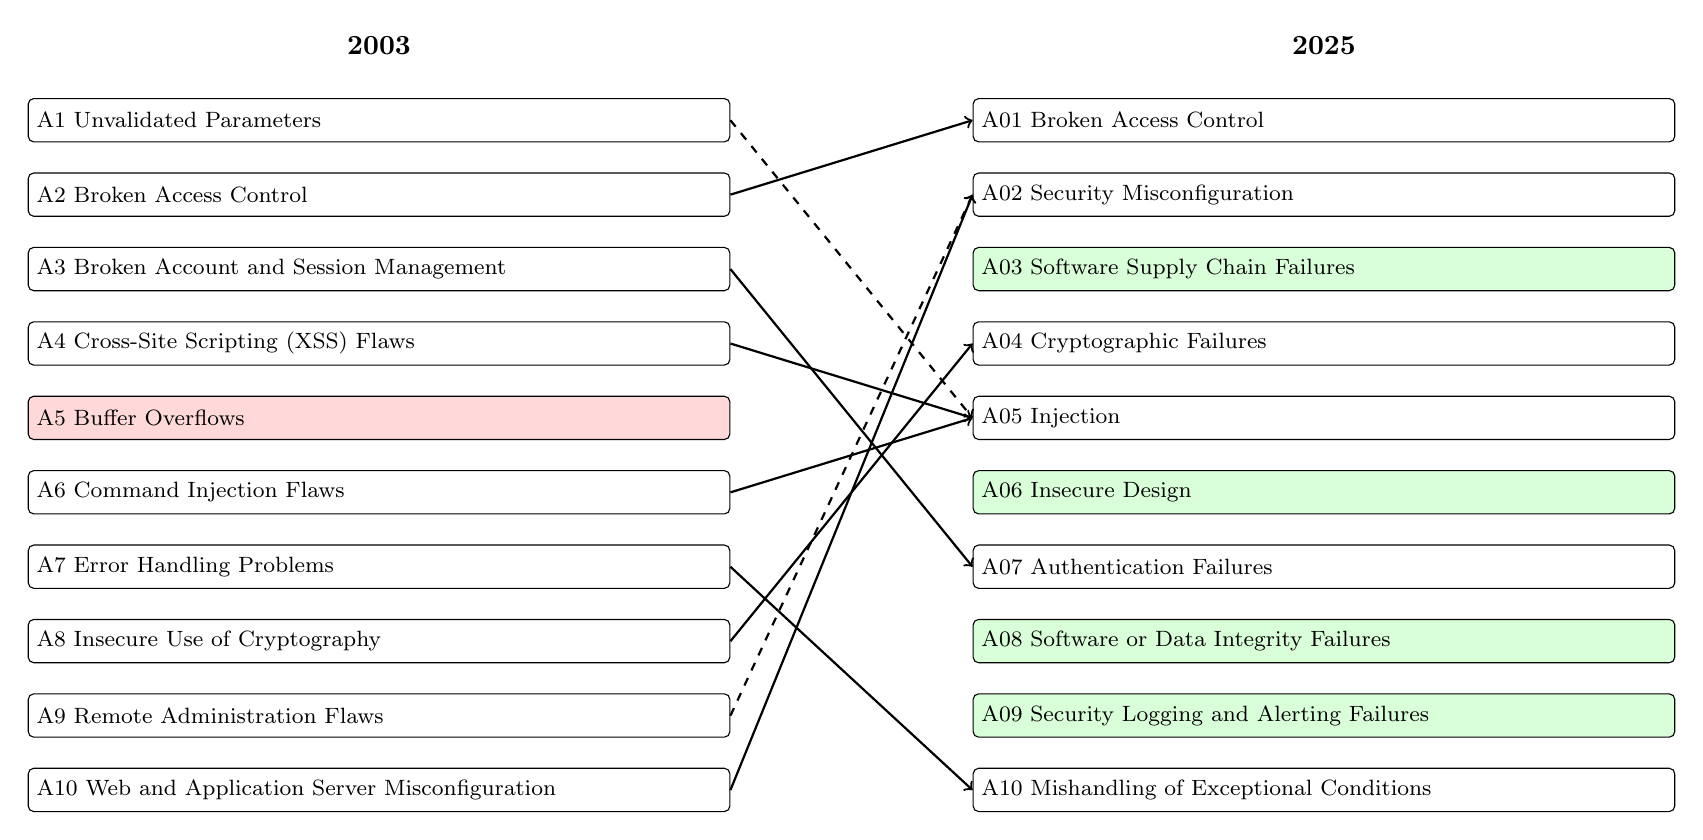
\begin{tikzpicture}[
  yscale=1.35,
  every node/.style={font=\footnotesize},
  item/.style={draw, rounded corners=2pt, text width=8.7cm, minimum height=0.55cm, inner sep=3pt},
  gone/.style={item, fill=red!15},
  new/.style={item, fill=green!15},
  map/.style={->, thick},
  loose/.style={->, thick, dashed}]

\node[font=\bfseries] at (0,0)  {2003};
\node[font=\bfseries] at (12,0) {2025};

\node[item] (o1)  at (0,-0.7) {A1 Unvalidated Parameters};
\node[item] (o2)  at (0,-1.4) {A2 Broken Access Control};
\node[item] (o3)  at (0,-2.1) {A3 Broken Account and Session Management};
\node[item] (o4)  at (0,-2.8) {A4 Cross-Site Scripting (XSS) Flaws};
\node[gone] (o5)  at (0,-3.5) {A5 Buffer Overflows};
\node[item] (o6)  at (0,-4.2) {A6 Command Injection Flaws};
\node[item] (o7)  at (0,-4.9) {A7 Error Handling Problems};
\node[item] (o8)  at (0,-5.6) {A8 Insecure Use of Cryptography};
\node[item] (o9)  at (0,-6.3) {A9 Remote Administration Flaws};
\node[item] (o10) at (0,-7.0) {A10 Web and Application Server Misconfiguration};

\node[item] (n1)  at (12,-0.7) {A01 Broken Access Control};
\node[item] (n2)  at (12,-1.4) {A02 Security Misconfiguration};
\node[new]  (n3)  at (12,-2.1) {A03 Software Supply Chain Failures};
\node[item] (n4)  at (12,-2.8) {A04 Cryptographic Failures};
\node[item] (n5)  at (12,-3.5) {A05 Injection};
\node[new]  (n6)  at (12,-4.2) {A06 Insecure Design};
\node[item] (n7)  at (12,-4.9) {A07 Authentication Failures};
\node[new]  (n8)  at (12,-5.6) {A08 Software or Data Integrity Failures};
\node[new]  (n9)  at (12,-6.3) {A09 Security Logging and Alerting Failures};
\node[item] (n10) at (12,-7.0) {A10 Mishandling of Exceptional Conditions};

\draw[loose] (o1.east)  -- (n5.west);
\draw[map]   (o2.east)  -- (n1.west);
\draw[map]   (o3.east)  -- (n7.west);
\draw[map]   (o4.east)  -- (n5.west);
\draw[map]   (o6.east)  -- (n5.west);
\draw[map]   (o7.east)  -- (n10.west);
\draw[map]   (o8.east)  -- (n4.west);
\draw[loose] (o9.east)  -- (n2.west);
\draw[map]   (o10.east) -- (n2.west);
\end{tikzpicture}
\end{center}

{\footnotesize Red: no longer on the list. Green: no 2003 counterpart. Dashed: loose mapping.
\link{https://owasp.org/Top10/2025/}}



\slide{CWE Common Weakness Enumeration}

\hlkimage{18cm}{cwe-mitre-org.png}
\link{http://cwe.mitre.org/}

\slide{CWE/SANS Monster mitigations}

\hlkimage{13cm}{cwe-monster-mitigations.png}

Source:
\link{http://cwe.mitre.org/top25/index.html}



\slide{Kubernetes hacker lab setup}

\hlkimage{6cm}{hacklab-1.png}

\begin{list2}
%\item Hardware: modern laptop CPU with virtualisation\\
%Dont forget to enable hardware virtualisation in the BIOS
%\item Software: your favourite operating system
\item Container and Virtualisation software: pick your own choice
\item Recommended RancherDesktop with Kubernetes as the the vulnerable systems
\item Hacker software: maybe a nearby Kali as a Virtual Machine \link{https://www.kali.org/}
\item Smallest Kubernetes: Minikube -  I have run this many times
\item Production deployment probably would use better tools like \faWrench\ \verb+Kubeadm+
\item Some instructions can be found at \link{https://codeberg.org/kramse/kramse-labs}
\end{list2}



\slide{OWASP Juice Shop Project}

\hlkimage{3cm}{JuiceShop_Logo_100px.png}

We will also use the OWASP Juice Shop Tool Project as a running example. This is an application which is modern AND designed to have security flaws.

Read more about this project at: \link{https://www.owasp.org/index.php/OWASP_Juice_Shop_Project}\\ \link{https://github.com/bkimminich/juice-shop}

Companion guide \emph{Pwning OWASP Juice Shop} \link{https://pwning.owasp-juice.shop}


\slide{Why Kubernetes / k3s?}

\hlkimage{17cm}{kubernetes-anywhere.png}

We often use a small local Kubernetes cluster (k3s, via Rancher Desktop) as the runtime for exercises. It gives everyone the same container-based exercise environment regardless of laptop OS (Windows, Mac, Linux).

\begin{list2}
  \item Faster to start, stop, and reset an exercise than a VM
  \item Same image runs identically on your laptop as it would in production
  \item Closer to how real-world applications are actually deployed and attacked today
%  \item Lets us study Kubernetes itself as an attack surface (misconfiguration, RBAC, kube-bench, etc.)
\end{list2}

%Why k3s specifically: a lightweight, single-binary Kubernetes distribution -- easy to run locally, low resource use, same API as "full" Kubernetes.
Read more at: \link{https://k3s.io/} and \link{https://kubernetes.io/}


\slide{Kubernetes Security is more than just the core}

\hlkimage{12cm}{rice-container-security-1.png}
Source: \emph{Container Security}, (CS) Liz Rice, O'Reilly, Apr 2020

\begin{list2}
\item Attacks from inside, attacks inside containers
\item Some just use up resources, some attacks others, some attack the system from the inside
\item Hacking Kubernetes have a whole \emph{Chapter 3 Container Runtime Isolation}
\end{list2}



\slide{Exercise: look up OWASP Juice Shop}

Try visiting the sites:
\begin{list2}
\item Project main site \link{https://owasp-juice.shop}
\item Source code \link{https://github.com/juice-shop/juice-shop}
\item Companion guide \emph{Pwning OWASP Juice Shop} \link{https://pwning.owasp-juice.shop}
\item Running Juice Shop on Kubernetes \link{https://codeberg.org/kramse/kramse-labs}
\end{list2}

Please spend a little time, look at the challenges in the companion guide and how they relate to the OWASP Top 10

Bookmark the sites for future reference.

\breakdance

\slide{Session 2: Security principles and design}
\begin{list2}
\item How to reach the goal of secure design
\item Security Principles for software
\item Principle of least privilege, fail-safe defaults, separation of privilege etc.
\item Security patterns, insecure and secure design
\vskip 1em
\item Exercise: least privilege -- everything runs as root\\
\end{list2}


\slide{Confidentiality, Integrity and Availability}

\hlkimage{8cm}{cia-triad-uk.pdf}

\begin{list1}
\item We want to protect something
\item Confidentiality - data kept a secret
\item Integrity - data is not subjected to unauthorized changes
\item Availability - data and systems are available when needed
\end{list1}

\slide{What is data?}
\hlkimage{5cm}{Linus3-04041999.jpg}

\begin{list1}
\item Personal data you dont want to loose:
\begin{list2}
\item Wedding pictures
\item Pictures of your children
\item Personal finances
\item Private information -- whatever that means for you
\end{list2}
\end{list1}

Source: picture of my son less than 24 hours old - precious!

\slide{Security is a process}

\begin{list1}
\item Remember:
\begin{list2}
\item what is information and security?
\item Data kept electronically
\item Data kept in physical form
\item Dont forget the human element of security
\end{list2}
\item Incident Response and Computer Forensics reaction to incidents
\item Good security is the result of planning and long-term work
\end{list1}
\vskip 1cm
\centerline{\color{titlecolor}\LARGE Security is a process, not a product, Bruce Schneier}

Source for quote: \link{https://www.schneier.com/essays/archives/2000/04/the_process_of_secur.html}


\slide{Work together}

\hlkimage{9cm}{Shaking-hands_web.jpg}

\begin{list1}
\item Team up!
\item We need to share security information freely
\item We often face the same threats, so we can work on solving these together
\end{list1}

\slide{Goals of Security}

\hlkimage{10cm}{incident-response-life-cycle.png}
{\footnotesize Source: \emph{Computer Security Incident Handling Guide}, NIST SP 800-61 Rev. 2}


\begin{list1}
\item Prevention - means that an attack will fail
\item Detection - determine if attack is underway, or has occured - report it
\item Recovery - stop attack, assess damage, repair damage
\end{list1}


\slide{Your data has already have been owned by criminals}

\hlkimage{13cm}{pwned.png}

\begin{list1}
\item Your data is already being sold, and resold on the Internet
\item Stop reusing passwords, use a password safe to generate and remember
\item Check you own email addresses on \link{https://haveibeenpwned.com/}
\end{list1}

\centerline{Go ahead try the web site - hold up your hand if you are in those dumps}



\slide{Balanced security}

\hlkimage{21cm}{afbalanceret-sikkerhed.pdf}

\begin{list1}
\item Better to have the same level of security
\item If you have bad security in some part - guess where attackers will end up
\item Hackers are not required to take the hardest path into the network
\item Realize there is no such thing as 100\% security
\end{list1}

\slide{Cost-Benefit Analysis}
% ROI?

\begin{list1}
\item Benefits of computer security must be weighed against value of assets
\item Often more expensive to add security mechanisms to a system, than designing them in
\end{list1}

\slide{Local vs. remote exploits}

\begin{list1}
\item {\bfseries Local vs. remote}
indicates whether an exploit targets
a vulnerability locally on the machine, for example
gaining higher privileges, or is intended
to exploit vulnerabilities over the network
\item {\bfseries Remote root exploit}
- the type most feared, since
it is an exploit program which, when run, gives
the attacker full control over the network -- root is the administrator
on Unix
\item {\bfseries Zero-day exploits} are those that are not published -- those
  hackers keep to themselves. Day 0 refers to nobody knowing
  about them before they are published, and often there are no fixes
  available for those vulnerabilities right away
\end{list1}

\slide{Security Princpiples}

We will use these as a reference:
\begin{list2}
\item The Protection of Information in Computer Systems is a 1975 seminal publication by Jerome Saltzer and Michael Schroeder about information security.[1][2] The paper emphasized that the primary concern of security measures should be the information on computers and not the computers itself.\\
\url{https://en.wikipedia.org/wiki/The_Protection_of_Information_in_Computer_Systems}
\item Principle of least privilege -- individual principles often have their own pages:\\
\url{https://en.wikipedia.org/wiki/Principle_of_least_privilege}
\item See also \emph{Security by Design Principles}\\
Selected as OWASP has existed for many years, expect site to survive\\
\url{https://www.owasp.org/index.php/Security_by_Design_Principles}
\end{list2}



\slide{Weak Structural Security}

Example design flaws:
\begin{list2}
\item Large Attack surface
\item Running a Process at Too High a Privilege Level, dont run everything as root or administrator
\item No Defense in Depth, use more controls, make a strong chain
\item Not Failing Securely
\item Mixing Code and Data
\item Misplaced trust in External Systems
\item Insecure Defaults
\item Missing Audit Logs
\end{list2}

\slide{Example applications from Microsoft}

How to get ahead? - use existing good examples!

Microsoft has released sample applications.

\begin{quote}
Secure Development Documentation
Learn how to develop and deploy secure applications on Azure with our sample apps, best practices, and guidance.

Get started
Develop a secure web application on Azure
\end{quote}

Source:
\url{https://docs.microsoft.com/en-us/azure/security/develop/}

Yes, this describes how to run Alpine Linux on their Azure Cloud.


\slide{Defense in depth}

%\hlkimage{10cm}{Bartizan.png}
\hlkimage{14cm}{medieval-clipart-5}
\centerline{Picture originally from: \url{http://karenswhimsy.com/public-domain-images}}



\slide{Defense in depth - layered security}

\hlkimage{5cm}{security-layers-1-uk.pdf}

\centerline{\hlkbig\color{security6blue} Multiple layers of security! Isolation!}



\slide{Principle of Least Privilege}

\begin{quote}
The \emph{principle of least privilege} states that a subject should be given only those privileges that it needs in order to complete the task.
\end{quote}
Source: \emph{Computer Security}, Matt Bishop, 2019

\begin{list2}
\item Originally formulated by Saltzer and Schroeder in 1975: every program and every user should operate with only the privileges needed for the job
\item Also drop privileges when not needed anymore, relinquish rights immediately
\item Example, need to read a document - but not write.
\item Database systems can often provide very fine grained access to data
\end{list2}

\slide{Principle of Fail-Safe defaults}

\begin{quote}
The \emph{principle of fail-safe defaults} states that, unless a subject is given explicit access to an object, it should be denied access to that object.
\end{quote}
Source: \emph{Computer Security}, Matt Bishop, 2019

\begin{list2}
\item Saltzer and Schroeder 1975: "Base access decisions on permission rather than exclusion"
\item Default access \emph{none}
\item In firewalls default-deny - that which is not allowed is prohibited
\item Newer devices today can come with no administrative users, while older devices often came with default admin/admin users
\item Real world example, OpenSSH \verb+PermitRootLogin+ -- root login with password is disabled by default
\end{list2}

\slide{Fail securely}

\begin{minted}[fontsize=\footnotesize]{java}
isAdmin = true;
try {
  codeWhichMayFail();
  isAdmin = isUserInRole( “Administrator” );
}
catch (Exception ex) {
  log.write(ex.toString());
}
\end{minted}
"If either codeWhichMayFail() or isUserInRole fails or throws an exception, the user is an admin by default. This is obviously a security risk."\\
Source: OWASP Security by Design Principles\\
\url{https://www.owasp.org/index.php/Security_by_Design_Principles}

\begin{list2}
\item DO use exception handling!
\item Just make sure code does not end up giving more privileges when failing!
\end{list2}



\slide{Separation of Duties and Function}

\begin{quote}
{\bf Separation of duties} (SoD; also known as Segregation of Duties) is the concept of having more than one person required to complete a task. In business the separation by sharing of more than one individual in one single task is an internal control intended to prevent fraud and error.
\end{quote}

Quote from \url{https://en.wikipedia.org/wiki/Separation_of_duties}

\begin{quote}
{\bf Separation of function}. Developers do not develop new programs on production systems because of the potential threat to production data.
\end{quote}
\emph{Computer Security}, Matt Bishop, 2019

Danish: Funktionsadskillelse


\slide{Role-based Access Control (RBAC)}

\begin{quote}
In computer systems security, {\bf role-based access control (RBAC)}[1][2] or role-based security[3] is an approach to restricting system access to unauthorized users. It is used by the majority of enterprises with more than 500 employees,[4] and can implement mandatory access control (MAC) or discretionary access control (DAC).

Role-based access control (RBAC) is a policy-neutral access-control mechanism defined around {\bf roles and privileges}. The components of RBAC such as role-permissions, user-role and role-role relationships make it simple to perform user assignments. A study by NIST has demonstrated that RBAC addresses many needs of commercial and government organizations[citation needed]. RBAC can be used to facilitate administration of security in large organizations with hundreds of users and thousands of permissions. Although RBAC is different from MAC and DAC access control frameworks, it can enforce these policies without any complication.
\end{quote}
Quote from \url{https://en.wikipedia.org/wiki/Role-based_access_control}



\slide{Example role based system: PostgreSQL security}
\hlkimage{15cm}{postgresql-security.png}

Feature overview security features in PostgreSQL\\
\url{https://www.postgresql.org/about/featurematrix/#security}


\slide{Security by Design}

\begin{list1}
\item All the principles today lead to {\bfseries Security by Design}
\begin{list2}
\item Secure defaults, minimize attack surface, fail securely
\item Least privilege -- no more "everything runs as root"
\item Security decisions are explicit choices, not accidents
\end{list2}
\item Applications don't run in a vacuum
\begin{list2}
\item They run in existing environments -- integrate with existing solutions, don't expect a clean slate
\item Make it easy to use by following conventions -- comply or explain why not
\end{list2}
\item Security from requirements and design to deployment
\begin{list2}
\item Threat modeling during design, checklists and cheat sheets to avoid repeating mistakes
\end{list2}
\end{list1}

Source: OWASP Developer Guide, 2.3 Principles of security and 4 Design\\
{\footnotesize\link{https://owasp.org/www-project-developer-guide/release/}}\\
See also: ENISA Secure by Design and Default Playbook



\slide{Breaking News: ENISA Secure by Design and Default Playbook}

{\bfseries\Large Hot off the press!} -- well, almost: published 30 July 2026

\begin{list1}
\item ENISA Secure by Design and Default Playbook\\
A Practical Guide to Secure by Design and Default Principles for SMEs
\begin{list2}
\item Principles turned into clear, repeatable actions
\item Fits into existing engineering, product and release processes
\item Covers the whole product life cycle
\item 22 playbooks, browsable on GitHub
\end{list2}
\item {\footnotesize\link{https://www.enisa.europa.eu/publications/enisa-secure-by-design-and-default-playbook}}
\item {\footnotesize\link{https://github.com/enisaeu/enisa-sbd-playbook/}}
\end{list1}

Today's principles are not old news -- the EU is still writing about them!

\slide{Stay Tuned: Where Security News Comes From}

\begin{list1}
\item The field moves -- the slides you see today will be outdated tomorrow
\item Follow the sources, not just the headlines:
\begin{list2}
\item OWASP -- Top 10, cheat sheets, Juice Shop\\
{\footnotesize\link{https://owasp.org}}
\item ENISA -- EU Agency for Cybersecurity, Cyber Resilience Act guidance\\
{\footnotesize\link{https://www.enisa.europa.eu/publications}}
\item NIST -- Secure Software Development Framework (SSDF), SP 800-218\\
{\footnotesize\link{https://csrc.nist.gov/projects/ssdf}}
\end{list2}
\item ENISA has an e-mail alert service -- sign up once, get the news delivered\\
{\footnotesize\link{https://www.enisa.europa.eu/alertservice}}
\end{list1}



\slide{Exercise: least privilege -- everything runs as root}

Two cases -- select the one that speaks most to you:
\begin{list1}
\item ERNW White Paper 68, Security Assessment of Cisco ACI\\{\footnotesize
\link{https://ernw.de/en/whitepapers/issue-68.html}}
\begin{list2}
\item 2.1 Remote Code Execution on Leaf Switches over IPv6 via Local SSH Server (CVE-2019-1836, CVE-2019-1803, and CVE-2019-1804)
\item 2.2.2 Cisco Nexus 9000 Series Fabric Switches Application Centric Infrastructure Mode Link Layer
Discovery Protocol Buffer Overflow Vulnerability (CVE-2019-1901)
\item 2.3 Cisco Application Policy Infrastructure Controller REST API Privilege Escalation Vulnerability (CVE-2019-1889)
\end{list2}
\item Cisco Secure Email Gateway SQL Injection, CVE-2026-76461\\{\footnotesize
\link{https://www.cisco.com/c/en/us/support/docs/csa/cisco-sa-esa-inj-2bLVGmhX.html}}
\end{list1}

Imagine you received this information being the developer:
Where is least privilege violated? Which CWE is it? \\
How serious would the vulnerability have been without root privileges?


\breakdance

\slide{Session 3: Code auditing, analysis and security testing}
\begin{list2}
\item Code-Auditing Strategies: static analysis and dynamic analysis
\item Security Testing Versus Traditional Software Testing
\vskip 1em
\item Exercise: clone OWASP Juice Shop and find the SQL injection\\
using grep or project search in your editor\\
\link{https://github.com/juice-shop/juice-shop}
% TODO: \exercise{} reference to existing exercise
\end{list2}



\slide{Hacker tools}

\begin{list1}
\item \emph{Improving the Security of Your Site by Breaking Into it}\\ by
Dan Farmer and Wietse Venema in 1993
\item Later in 1995 release the software SATAN\\
\emph{Security Administrator Tool for Analyzing Networks}
\item Caused some commotion, panic and discussions, every script kiddie can hack, the internet will melt down!
\vskip 5mm
\begin{quote}
We realize that SATAN is a two-edged sword -- like
many tools, it can be used for good and for evil
purposes. We also realize that intruders (including
wannabees) have much more capable (read intrusive)
tools than offered with SATAN.
\end{quote}
\end{list1}

\vskip 1cmlabel
Source:
\link{http://www.fish2.com/security/admin-guide-to-cracking.html}


\slide{Use hacker tools!}

\begin{list1}
\item Port scan can reveal holes in your defense
\item Web testing tools can crawl through your site and find problems
\item Pentesting is a verification and proactively finding problems
\item Its not a silverbullet and mostly find known problems in existing systems
\item Combined with honeypots they may allow better security
\end{list1}




\slide{Testing - more work now, less work in the long run}

% noget QA relateret, måske logo fra Hudson?
%checkmark
\hlkimage{12cm}{testing.pdf}


\slide{Unit testing - low level / functions}

\begin{minted}[fontsize=\small]{java}
public class TestAdder {
    public void testSum() {
        Adder adder = new AdderImpl();
        assert(adder.add(1, 1) == 2);
        assert(adder.add(1, 2) == 3);
        assert(adder.add(2, 2) == 4);
        assert(adder.add(0, 0) == 0);
        assert(adder.add(-1, -2) == -3);
        assert(adder.add(-1, 1) == 0);
        assert(adder.add(1234, 988) == 2222);
    }
}
\end{minted}

\begin{list1}
\item Test individual functions
\item Example from \link{http://en.wikipedia.org/wiki/Unit_testing}
\item Avoid regressions, old errors reappearing
\end{list1}

\slide{Analysis}

%\hlkimage{10cm}{Magnifying_Glass.png}
\hlkimage{12  cm}{buffer-overflow-3.pdf}

\centerline{Use tools for analysing code and applications}

\slide{Typer af analyse}

\begin{list1}
\item  {\Large statisk analyse}\\
finder fejl uden at køre programmet\\
typisk findes konstruktioner som indeholder fejl, brug af forkerte funktioner m.v.
\item {\Large dynamisk analyse}\\
findes ved at køre programmet, typisk i et specielt miljø
\end{list1}

\slide{Statiske analyseværktøjer}
\begin{list1}
\item Flawfinder \link{http://www.dwheeler.com/flawfinder/}
\item RATS Rough Auditing Tool for Security, C, C++, Perl, PHP and Python
\item PMD static ruleset based Java
\item {\small \link{http://en.wikipedia.org/wiki/List_of_tools_for_static_code_analysis}}
\end{list1}

\slide{A Fool with a Tool is still a Fool}

\begin{list1}
\item 1. Run tool
\item 2. Fix problems
\item 3. Rinse repeat
\end{list1}

Fixing problems?\\
\begin{minted}[fontsize=\small]{c}
   char tmp[256]; /* Flawfinder: ignore */
   strcpy(tmp, pScreenSize); /* Flawfinder: ignore */
\end{minted}
Eksempel fra \link{http://www.dwheeler.com/flawfinder/}


\slide{Pseudo Random Number Generator}

\hlkimage{21cm}{debian-prng.png}

{\small\link{https://en.wikipedia.org/wiki/Random_number_generator_attack\#Debian_OpenSSL}}

\vskip 1cm
\centerline{The random number generator is VITAL for crypto security}




\slide{Hard to do -  manual analysis}

\begin{list1}
\item Hvorfor ikke bare programmere sikkert?
\item Der er mange ressourcer tilgængelige:
\item Websites: \emph{Secure Programming for Linux and Unix HOWTO }\\
\link{http://www.dwheeler.com/secure-programs/}
\item Bøger: \emph{24 Deadly Sins of Software Security: Programming Flaws and How to Fix Them }
Michael Howard, David LeBlanc, John Viega + deres andre bøger

\end{list1}

\vskip 2cm
\centerline{\Large Det er for svært, dyrt, tager for lang tid!?}


\slide{Dynamic analysis}

%http://www.onjava.com/pub/a/onjava/2003/02/12/static_analysis.html

\begin{list1}
\item compile time vs. at run time nogle fejl kan ikke findes på compile-time
\item Er du doven så oversæt og kør programmet på OpenBSD ;-)
\end{list1}


\slide{Break it}


\hlkimage{12cm}{300px-Fozziecurtain.JPG}

\centerline{Use fuzzers, hackertools, improve security by breaking it}


\slide{Simple fuzzer}

\begin{alltt}
$ for i in 10 20 30 40 50
>> do
>> ./demo `perl -e "print 'A'x$i"`
>> done
AAAAAAAAAA
AAAAAAAAAAAAAAAAAAAA
AAAAAAAAAAAAAAAAAAAAAAAAAAAAAA
Memory fault
AAAAAAAAAAAAAAAAAAAAAAAAAAAAAAAAAAAAAAAA
Memory fault
AAAAAAAAAAAAAAAAAAAAAAAAAAAAAAAAAAAAAAAAAAAAAAAAAA
Memory fault
\end{alltt}

\centerline{Memory fault/segmentation fault - juicy!}



\slide{Enhance and secure runtime environment}

%\hlkimage{10cm}{Bartizan.png}
\hlkimage{15cm}{medieval-clipart-5}
%\centerline{Picture from: http://karenswhimsy.com/public-domain-images}

\centerline{Sidste chance er på afviklingstidspunktet}



\slide{Chroot, Jails and }

\begin{list1}
\item Der findes mange typer \emph{jails} på Unix
\item Ideer fra Unix chroot som ikke er en egentlig sikkerhedsfeature
\begin{list2}
\item Unix chroot - bruges stadig, ofte i daemoner som OpenSSH
\item FreeBSD Jails
\item SELinux
\item Solaris Containers og Zones - \emph{jails på steroider}
\item VMware virtuelle maskiner, er det et jail?
\end{list2}
\item Hertil kommer et antal andre måder at adskille processer - sandkasser
\item Husk også de simple, database som \verb+_postgresql+, Tomcat som \verb+tomcat+, Postfix postsystem som \verb+_postfix+, SSHD som \verb+sshd+ osv. - simple brugere, få rettigheder
\end{list1}

\slide{JVM security policies}

\begin{minted}[fontsize=\small]{java}
// ========== WEB APPLICATION PERMISSIONS =====================================
// These permissions are granted by default to all web applications
// In addition, a web application will be given a read FilePermission
// and JndiPermission for all files and directories in its document root.
grant {
    // Required for JNDI lookup of named JDBC DataSource's and
    // javamail named MimePart DataSource used to send mail
    permission java.util.PropertyPermission "java.home", "read";
    permission java.util.PropertyPermission "java.naming.*", "read";
    permission java.util.PropertyPermission "javax.sql.*", "read";
...
};
// The permission granted to your JDBC driver
// grant codeBase "jar:file:${catalina.home}/webapps/examples/WEB-INF/lib/driver.jar!/-" \{
//      permission java.net.SocketPermission "dbhost.mycompany.com:5432", "connect";
// \};
\end{minted}

\begin{list1}
\item Eksempel fra \verb+apache-tomcat-6.0.18/conf/catalina.policy+
\end{list1}


\slide{Apple sandbox named generic rules}

\begin{minted}[fontsize=\small]{lisp}
;; named - sandbox profile
;; Copyright (c) 2006-2007 Apple Inc.  All Rights reserved.
;;
;; WARNING: The sandbox rules in this file currently constitute
;; Apple System Private Interface and are subject to change at any time and
;; without notice. The contents of this file are also auto-generated and not
;; user editable; it may be overwritten at any time.
;;
(version 1)
(debug deny)

(import "bsd.sb")

(deny default)
(allow process*)
(deny signal)
(allow sysctl-read)
(allow network*)
\end{minted}


\slide{Apple sandbox named specific rules }

\begin{minted}[fontsize=\small]{lisp}
;; Allow named-specific files
(allow file-write* file-read-data file-read-metadata
  (regex "^(/private)?/var/run/named\\pid$"
         "^/Library/Logs/named\\.log$"))

(allow file-read-data file-read-metadata
  (regex "^(/private)?/etc/rndc\\.key$"
         "^(/private)?/etc/resolv\\.conf$"
         "^(/private)?/etc/named\\.conf$"
         "^(/private)?/var/named/"))
\end{minted}

\begin{list1}
\item Eksempel fra \verb+/usr/share/sandbox+ på Mac OS X
\end{list1}



\breakdance

\slide{Session 4: Coding standards, Git hooks and scanner tools}
\begin{list2}
\item Policies, coding standards, compiler warnings, defensive programming
\item Git hooks and scanner integration in continuous integration
\item Tools: Semgrep, Bandit, Ruff
\vskip 1em
\item Exercise: research Semgrep as Git hook and CI tool\\
\link{https://semgrep.dev/docs/extensions/pre-commit}\\
Discuss: which tools does your team run today -- locally, in hooks or in CI?
\end{list2}


\slide{Introduction to Methods}

\begin{list2}
\item Following slides list some of the methods for eliminating security issues
\item Sometimes when eliminating is not possible the runtime environment can be improved
\item Other times the strategy involves the systems used for development - like alleviating the version control systems to enforce policies and restrict developers from doing bad things
\end{list2}

\slide{Low hanging fruits - easy }

%billede af nogle frugter
\hlkimage{10cm}{38-line-drawing-of-a-pare-fruit.png}

\centerline{Higher quality software is often more secure}

\slide{Coding standards - style}

\begin{quote}
This file specifies the preferred style for kernel source files in the
OpenBSD source tree.  It is also a guide for preferred user land code
style.  These guidelines should be followed for all new code.  In general,
code can be considered ``new code'' when it makes up about 50% or
more of the file(s) involved. ...\\
Use queue(3) macros rather than rolling your own lists, whenever possible.
Thus, the previous example would be better written:
\end{quote}

\begin{minted}[fontsize=\small]{c}
    #include <sys/queue.h>
    struct  foo {
    LIST_ENTRY(foo) link;  /* Queue macro glue for foo lists */
               struct  mumble amumble; /* Comment for mumble */
               int     bar;
    };
    LIST_HEAD(, foo) foohead;     /* Head of global foo list */
\end{minted}


OpenBSD style(9)

\slide{Coding standards functions}

\begin{quote}
The following copies as many characters from input to buf as will fit and
NUL terminates the result.  Because strncpy() does not guarantee to NUL
terminate the string itself, it must be done by hand.
\end{quote}

\begin{minted}[fontsize=\small]{c}
        char buf[BUFSIZ];

        (void)strncpy(buf, input, sizeof(buf) - 1);
        buf[sizeof(buf) - 1] = '\0';
\end{minted}

\begin{quote}
Note that \verb+strlcpy(3)+ is a better choice for this kind of operation.  The
equivalent using \verb+strlcpy(3)+ is simply:
\end{quote}
\begin{minted}[fontsize=\small]{c}
        (void)strlcpy(buf, input, sizeof(buf));
\end{minted}

OpenBSD strcpy(9)

\slide{Compiler warnings - gcc -Wall}

\begin{minted}[fontsize=\small]{bash}
# gcc -o demo demo.c
demo.c: In function main:
demo.c:4: warning: incompatible implicit declaration of built-in
function strcpy
\end{minted}

\begin{minted}[fontsize=\small]{bash}
# gcc -Wall -o demo demo.c
demo.c:2: warning: return type defaults to int
demo.c: In function main:
demo.c:4: warning: implicit declaration of function strcpy
demo.c:4: warning: incompatible implicit declaration of built-in
function strcpy
demo.c:5: warning: control reaches end of non-void function
\end{minted}

\vskip 15mm
\centerline{\bf\LARGE\color{security6blue}Easy to do!}

\slide{No warnings = no errors?}

\begin{minted}[fontsize=\small]{c}
# cat demo2.c
#include <strings.h>
int main(int argc, char **argv)
{
    char buf[200];
    strcpy(buf, argv[1]);
    return 0;
}
# gcc -Wall -o demo2 demo2.c
\end{minted}

\vskip 1cm
\centerline{\bf\large\color{security6blue}This is an insecure program, but no warnings!}

(cheating, some compilers actually warn today)



\slide{Version control sample hooks scripts}

\begin{list1}
\item Before checking in code in version control,  pre-commit - check
\begin{list2}
\item case-insensitive.py
\item check-mime-type.pl
\item commit-access-control.pl
\item commit-block-joke.py
\item detect-merge-conflicts.sh
\item enforcer
\item log-police.py
\item pre-commit-check.py
\item verify-po.py
\end{list2}
\item \link{http://subversion.tigris.org/tools_contrib.html}
\item \link{http://svn.collab.net/repos/svn/trunk/contrib/hook-scripts/}
\end{list1}

This references Subversion, which is not used much anymore. Just to show the concept is NOT new. Use hooks!

\slide{Example Enforcer}

\begin{alltt}
In a Java project I work on, we use log4j extensively.  Use of
System.out.println() bypasses the control that we get from log4j,
so we would like to discourage the addition of println calls in
our code.

We want to deny any commits that add a println into the code.
The world being full of exceptions, we do need a way to allow
some uses of println, so we will allow it if the line of code
that calls println ends in a comment that says it is ok:

   System.out.println("No log4j here"); // (authorized)
\end{alltt}

{\small \link{http://svn.collab.net/repos/svn/trunk/contrib/hook-scripts/enforcer/enforcer}}



\slide{Example verify-po.py}

\begin{minted}[fontsize=\small]{python}
#!/usr/bin/env python
"""This is a pre-commit hook that checks whether the contents
of PO files committed to the repository are encoded in UTF-8.
"""
\end{minted}

{\small \link{http://svn.collab.net/repos/svn/trunk/tools/hook-scripts/verify-po.py}}

\slide{Design for security - more work}

\hlkimage{14cm}{johnny_automatic_blueprints.png}
\centerline{Security is cheapest and most effective when done during design phase.}



\breakdance

\slide{Session 5: Secure Development Lifecycle and standards}
\begin{list2}
\item Secure Development Lifecycle (SDL, SDLC, SSDL) -- multiple names, but essentially the same
\item Standards ISO 27001/CIS Controls, Application Software Security
\item ISO/IEC 27001:2022 Annex A 8.25--8.31
\vskip 1em
\item Exercise: your processes and documentation vs.\ Annex A -- where are the gaps?\\
Continues in the optional part at the end of the day
\end{list2}


\slide{Design for security - more work}

\hlkimage{14cm}{johnny_automatic_blueprints.png}
\centerline{Security is cheapest and most effective when done during design phase.}



\slide{Secure Coding starts with the design}

%\hlkimage{5cm}{secure_coding.png}

\vskip 2cm
\hlkrightimage{4cm}{secure_coding.png}
{\emph{Secure Coding: Principles and Practices} af Mark G. Graff, Kenneth R. Van Wyk 2003}



\begin{list1}
\item Architecture/design -- while you are thinking about the application
\item Implementation -- while you are writing the application
\item Operations -- After the application is in production
\item Ca. 200 pages, very dense.
\end{list1}


\slide{Design a robust network Isolation and segmentation}

\begin{list1}
\item What can you do to improve network security?
\begin{list2}
\item Use switches -- sniffing then requires ARP spoofing, and better performance
\item Divide with firewalls into multiple DMZ zones to keep
      exposed servers separated from each other, the internal network and
      the Internet
\item Monitor, read logs and respond to incidents
\end{list2}
\item Remember you also need to be able to update your servers
\end{list1}

\slide{Basic Network Security Pattern Isolate in VLANs}

\hlkimage{10cm}{images/demo-netvaerk.pdf}

\begin{list1}
\item You should segment your network based on traffic
\item You should always keep internal and external systems separated!
\item You should isolate dangerous services in jails and chroots
\item Use port security to protect basic services like DHCP, Spanning Tree etc.
\end{list1}

\slide{Building Secure Infrastructures}

\begin{list1}
\item A real-life setup of an infrastructure from scratch can be daunting!
\item You need:
\begin{list2}
\item Policies
\item Procedures
\item Incident Response
\end{list2}
\item Running systems which require
\begin{list2}
\item Configurations
\item Settings
\item Supporting infrastructure -- networks
\item Supporting infrastructure -- logging, dashboarding, monitoring
\end{list2}
\item Building something \emph{secure} is {\bf hard work!}
\end{list1}



\slide{Existing infrastructures}

\begin{list1}
\item or even worse you inherited an infrastructure
\item Multiple networks, with different vendors, rules
\item Multiple generations of services, applications, technologies
\item Built over decades
\item Varying to no documentation
\item Organizational challenges
\item Ingrained culture -- frozen in time
\end{list1}

How do you get started improving security?

\slide{Integrate or develop?}

\begin{list1}
\item Dont:
\begin{list2}
\item Reinvent the wheel - too many times, unless you can maintain it afterwards
\item Never invent cryptography yourself
\item No copy paste of functionality, harder to maintain in the future
\end{list2}
\item Do:
\begin{list2}
\item Integrate with existing solutions
\item Use existing well-tested code: cryptography, authentication, hashing
\item Centralize security in your code and organization
\end{list2}
\end{list1}



\slide{ISO/IEC 27001:2022 Information Security Management Systems}

\begin{list2}
\item ISO/IEC 27001:2022 specifies requirements for an Information Security Management System (ISMS)
\item Annex A lists 93 reference controls, grouped in four themes:\\
5 Organizational (37), 6 People (8), 7 Physical (14), 8 Technological (34)
\item ISO/IEC 27002:2022 gives implementation guidance for each control
\item The organization decides which controls apply, based on risk assessment\\
-- documented in the Statement of Applicability (SoA)
\item Excluding a control requires a justification\\
"We don't develop software" is often not a valid reason -- scripts, automation and configuration count too
\end{list2}

Source: ISO/IEC 27001:2022, ISO/IEC 27002:2022

\slide{Annex A -- Secure Development Controls}

\begin{list2}
\item 8.25 Secure development life cycle
\item 8.26 Application security requirements
\item 8.27 Secure system architecture and engineering principles
\item 8.28 Secure coding
\item 8.29 Security testing in development and acceptance
\item 8.30 Outsourced development
\vskip 1em
\item Your ISMS project has to answer for each: does it apply, and how do we meet it?
\item The following slides: what the control asks for (paraphrased), and questions to ask in your organization
\end{list2}

Source: ISO/IEC 27001:2022 Annex A

\slide{Secure Development Life Cycle}

\begin{quote}
Control 8.25:\\
Secure development life cycle\\
Rules for secure development of software and systems are established and applied. (paraphrased)
\end{quote}

\begin{list1}
\item Do we have a documented secure development policy?
\item Which phases of our development process include security activities?
\item Who is responsible for security in each phase?
\item Are developers trained in secure development?
\end{list1}

Source: ISO/IEC 27001:2022 Annex A 8.25, see also Session 5 SDL/SSDL

\slide{Application Security Requirements}

\begin{quote}
Control 8.26:\\
Application security requirements\\
Information security requirements are identified, specified and approved when developing or acquiring applications. (paraphrased)
\end{quote}

\begin{list1}
\item Where do our security requirements come from -- risk assessment, legislation, GDPR, customers?
\item How are they written down -- user stories, abuse cases, checklists?
\item Who approves them, and when in the project?
\item Do we use a reference, e.g.\ OWASP Top 10 or OWASP ASVS?
\end{list1}

Source: ISO/IEC 27001:2022 Annex A 8.26, see also Session 1 OWASP

\slide{Secure System Architecture and Engineering Principles}

\begin{quote}
Control 8.27:\\
Secure system architecture and engineering principles\\
Principles for engineering secure systems are established, documented, maintained and applied to all development. (paraphrased)
\end{quote}

\begin{list1}
\item Which security principles do we follow -- least privilege, fail-safe defaults, defense in depth?
\item Are they written down, or only in people's heads?
\item Do we do design reviews or threat modelling before implementation?
\item Would our products pass the "everything runs as root" test?
\end{list1}

Source: ISO/IEC 27001:2022 Annex A 8.27, see also Session 2 principles and design

\slide{Secure Coding}

\begin{quote}
Control 8.28:\\
Secure coding\\
Secure coding principles are applied to software development. (paraphrased)
\end{quote}

\begin{list1}
\item Do we have coding standards, and are they enforced?
\item Compiler warnings, linters and scanners -- e.g.\ Ruff, Bandit, Semgrep?
\item Git hooks and CI -- what is checked before code is merged?
\item Code review -- does it include security, and who does it?
\end{list1}

Source: ISO/IEC 27001:2022 Annex A 8.28, see also Session 4 coding standards and tools

\slide{Security Testing in Development and Acceptance}

\begin{quote}
Control 8.29:\\
Security testing in development and acceptance\\
Security testing processes are defined and implemented in the development life cycle. (paraphrased)
\end{quote}

\begin{list1}
\item Which security tests run automatically -- static and dynamic analysis?
\item Do acceptance criteria include security requirements from 8.26?
\item Penetration testing before go-live -- when, by whom?
\item How are findings tracked and fixed?
\end{list1}

Source: ISO/IEC 27001:2022 Annex A 8.29, see also Session 3 code auditing and testing

\slide{Outsourced Development}

\begin{quote}
Control 8.30:\\
Outsourced development\\
The organization directs, monitors and reviews activities related to outsourced system development. (paraphrased)
\end{quote}

\begin{list1}
\item Do contracts with suppliers include security requirements?
\item Do we have the right to audit, or to see test results?
\item How do we verify delivered code -- same scanners and tests as our own?
\item Third-party libraries and dependencies -- who is responsible for them?
\end{list1}

Source: ISO/IEC 27001:2022 Annex A 8.30

\slide{Annex A Controls and This Course}

\begin{list2}
\item 8.25 Secure development life cycle -- Session 5
\item 8.26 Application security requirements -- Session 1, OWASP Top 10
\item 8.27 Secure system architecture and engineering principles -- Session 2
\item 8.28 Secure coding -- Session 4
\item 8.29 Security testing in development and acceptance -- Session 3
\item 8.30 Outsourced development -- discussion in this session
\vskip 1em
\item The controls describe {\bf what} -- the course has shown examples of {\bf how}
\end{list2}

\slide{Exercise: Where Are Our Gaps?}

\begin{list2}
\item In groups, go through 8.25--8.30 using the questions on the previous slides
\item For each control:
\begin{list1}
\item What do we already do -- process, tools, documentation?
\item What is missing or only informal?
\item What would be the first concrete step?
\end{list1}
\item Use what you shared in Session 4 about the tools you run today
\item Continues in the optional part at the end of the day
\end{list2}

I invite you to reflect on today's subjects, and how they can help mature your development work.

\breakdance

% Lesson 6
\slide{Part 7: Optional: Exercises, questions}



\slide{Prerequisites}

\begin{list2}
\item I recommend doing exercises
\item I use Linux and Kubernetes, but previous Linux and Unix knowledge is not needed
\item It is recommended to use containers and virtual machines for the exercises
\item Web security is a great example since the web server runs on top of operating systems and lower, plus it runs application frameworks, code by the developers etc

\item Security and most internet related security work has the following requirements:\\
Network experience, Server experience, TCP/IP principles - often in more detail than a common user, Programming is an advantage, for automating things
\end{list2}

\slide{More than half of Microsoft Azure Cloud runs Linux}

%\hlkimage{}{}

\begin{quote}
{\large Run Linux virtual machines (VMs) on Azure}

Efficiently run Linux workloads on Azure with built-in security and management

More than 60\% of customer cores in Azure run Linux workloads. Choose from popular Linux distributions including Red Hat, SUSE, Ubuntu, Debian, Flatcar, and Oracle Linux. Use preconfigured solutions from Oracle and other open-source VM-compatible providers and find Azure-optimized Linux VM images from publishers of your choice.
\end{quote}
Source: \url{https://azure.microsoft.com/en-us/products/virtual-machines/linux}



\slide{Analysis on Docker Hub malicious images}

\hlkimage{10cm}{sysdig-malicious-images.png}
This article is relevant, talking about malicious docker images\\
\link{https://sysdig.com/blog/analysis-of-supply-chain-attacks-through-public-docker-images/}



\slide{Benchmarking tools}

\begin{quote}
\faWrench\ \verb+Kube-bench+ is the industry-standard tool to automate checking Kubernetes compliance with the Center for Internet Security (CIS) Benchmark.

Kube-bench makes it easy for operators to check whether each node in their Kubernetes cluster is configured according to security best practices.
\end{quote}
Source: \link{https://info.aquasec.com/open-source}

\begin{list2}
\item CIS Kubernetes V1.24 Benchmark v1.0.0 - 09-21-2022 -- other versions exist
\item CIS Docker Benchmark v1.5.0 - 12-28-2022
\end{list2}

%\slide{Benchmarking and keeping up to date}

% Try it out \faWrench\ \verb+kube-bench+ - make some bad changes, like LKS p95 allow anonymous authentication, show why layered defense works, and how kube-bench marks it. Another example token based access, initially we have token while installing, remember to remove!
% \faWrench\ \verb+kube-hunter+ and kube-bench

\slide{Tool example kube-bench}

%\hlkimage{}{}

\begin{alltt}\scriptsize
hlk@timon:~/bin/kube-bench/kube-bench$ {\bf kubectl logs kube-bench-gdf62}
[PASS] 1.1.7 Ensure that the etcd pod specification file permissions are set to 600 or more restrictive (Automated)
[PASS] 1.1.8 Ensure that the etcd pod specification file ownership is set to root:root (Automated)
[WARN] 1.1.9 Ensure that the Container Network Interface file permissions are set to 600 or more restrictive (Manual)
[WARN] 1.1.10 Ensure that the Container Network Interface file ownership is set to root:root (Manual)
[PASS] 1.1.11 Ensure that the etcd data directory permissions are set to 700 or more restrictive (Automated)
[FAIL] 1.1.12 Ensure that the etcd data directory ownership is set to etcd:etcd (Automated)
...
== Summary policies ==
0 checks PASS
0 checks FAIL
35 checks WARN
0 checks INFO

== Summary total ==
63 checks PASS
10 checks FAIL
58 checks WARN
0 checks INFO

\end{alltt}

\begin{list2}
\item \url{https://github.com/aquasecurity/kube-bench} also check out Lynis \url{https://cisofy.com/lynis/}
\end{list2}




\slide{Kubernetes hacker lab setup}

\hlkimage{6cm}{hacklab-1.png}

\begin{list2}
%\item Hardware: modern laptop CPU with virtualisation\\
%Dont forget to enable hardware virtualisation in the BIOS
%\item Software: your favourite operating system
\item Container and Virtualisation software: pick your own choice
\item Recommended RancherDesktop with Kubernetes as the the vulnerable systems
\item Hacker software: maybe a nearby Kali as a Virtual Machine \link{https://www.kali.org/}
\item Smallest Kubernetes: Minikube -  I have run this many times
\item Production deployment probably would use better tools like \faWrench\ \verb+Kubeadm+
\item Some instructions can be found at \link{https://codeberg.org/kramse/kramse-labs}
\end{list2}




% \demo{ex:sw-basicLinuxetc}


\demo{ex:prepare-for-course}
\demo{ex:git-tutorial}

\demo{ex:sw-kubernetes}

\demo{ex:sw-startjuice}


\demo{ex:js-burp}

\demo{ex:sw-kubebench-k3s}
\demo{ex:sw-trivy-k3s}

\demo{ex:juiceshop-attack}
\demo{ex:truncate-encoding}
\demo{ex:juice-shop-login}


\end{document}
